\chapter{Background}
\label{chapter:Background}
This chapter provides the necessary theoretical an technological background topics of the thesis.

\section{Axioms of Linguistic Architectures}
\label{section:AxiomsOfLinguisticArchitectures}
This section summarizes axioms of linguistics architectures.
Axioms are outlined in \cite{DBLP:conf/sle/Lammel16} and refined in \cite{DBLP:conf/modelsward/HeinzLV17}.
§\ref{subsection:Parthood} introduces the axiomatization for \gls{Parthood}
§\ref{subsection:Fragments} 

Axioms are presented in First Order Logic and formalization is taken from \cite{DBLP:conf/modelsward/HeinzLV17}.
The universe to draw elements from is represented by the \Entity-predicate:
\begin{align*}
\forall x.\Entity(x).\qquad\text{\cite{DBLP:conf/modelsward/HeinzLV17}}
\end{align*}
We assume it holds for everything of interest, hence such things are called \textit{entities}.

Linguistic architectures intend to describe software from language centric point of view, thus we provide specializations of entities for languages:
\begin{align*}
&\Set(x) \Rightarrow \Entity(x).
&\text{\cite{DBLP:conf/modelsward/HeinzLV17}}
\\
&\Language(x) \Rightarrow \Set(x).
&\text{\cite{DBLP:conf/modelsward/HeinzLV17}}
\end{align*}
There are entities representing sets in a mathematical sense, and there are sets representing (formal-) languages in the sense of theoretical computer science.

On the other hand, we provide specializations for entities involved in software engineering terminology:
\begin{align*}
&\Artifact(x) \Rightarrow \Entity(x).
&\text{\cite{DBLP:conf/modelsward/HeinzLV17}}
\\
&\File(x) \Rightarrow \Artifact(x).
&\text{\cite{DBLP:conf/modelsward/HeinzLV17}}
\\
&\Folder(x) \Rightarrow \Artifact(x).
&\text{\cite{DBLP:conf/modelsward/HeinzLV17}}
\end{align*}
There are entities representing all kinds of digital artifacts, e.g. files and folders.
Files represent persistent data resources, locatable either trough file systems or web services.
Folders represent locatable collections of files.
The intended use and semantic of these predicates is not meant to differ from intuitive, every day use.


\subsection{Parthood}
\label{subsection:Parthood}
\Gls{Parthood} is the essential relationship when reasoning about \gls{Correspondence} and \gls{Conformance} among artifacts within linguistic architectures \cite{DBLP:conf/sle/Lammel16} \cite{DBLP:conf/modelsward/HeinzLV17}.
It describes the relation between entities and their constituent parts.
The study of \gls{Parthood} and its derivatives is \gls{Mereology} \cite{DBLP:journals/dke/Varzi96} \cite{SEP:Mereology}.
In the context of linguistic architectures we assume most entities to be
composed of several conceptual or "physical"\footnote{We mean physical in the sense, that an entity manifests in some (digital) form, but not in the sense that someone can touch it with bare hands} parts.
In short, such entities exists as sum of their parts.
That is, programs may compiled from many files, systems consists of several disjoint but dependent components, a \gls{Java} class is made up of methods and fields, etc.
Furthermore such entities are considered to be \textit{mereologically invariant}, i.e. if one part changes, the whole changes as well. 
Axiom \ref{axiom:PartOf} captures \gls{Parthood} at its most basic level.
\begin{axiom}[\partOf]
\label{axiom:PartOf}
\begin{align*}
&\partOf(p,w)
\Rightarrow
\Entity(p) \wedge \Entity(w).\\
&\partOf(p,w)
\Leftarrow
p \text{ is a constituent part of } w.
\end{align*}
\end{axiom}
The formalization presented here is not taken from \cite{DBLP:conf/modelsward/HeinzLV17}, where it is not formalized explicitly, nor is it directly taken from \cite{DBLP:conf/sle/Lammel16}.
It is rather a byproduct of merging works on \glspl{LinguisticArchitecture} with works on \gls{Mereology} (see \cite{DBLP:conf/sle/Lammel16} \cite{DBLP:conf/modelsward/HeinzLV17} and \cite{DBLP:journals/dke/Varzi96} \cite{SEP:Mereology} respectively). 
\Gls{Parthood} is usually considered to be reflexive, antisymmetric and transitive, thus facilitating a partial order \cite{DBLP:journals/dke/Varzi96} \cite{SEP:Mereology}:
\begin{align*}
&\partOf(p,p).
&\text{Reflxivity}
\\
&\partOf(p,w) \wedge \partOf(w,p) \Rightarrow p = w. 
&\text{Antisymmertry}
\\
&\partOf(p,w) \wedge \partOf(w,u) \Rightarrow \partOf(p,u). 
&\text{Transitivity}
\end{align*}
Other authors consider \partOf~ to be stricter, e.g. \cite{DBLP:conf/sle/Lammel16}, tending towards an irreflexive \gls{Parthood} relationship.
Irreflexive \gls{Parthood} is called proper in context of \gls{Mereology} \cite{DBLP:journals/dke/Varzi96} \cite{SEP:Mereology}:
\begin{align*}
&\properPartOf(p,w)
\Rightarrow
\Entity(p) \wedge \Entity(w).\\
&\properPartOf(x,y)
\Leftarrow
\partOf(x,y) \wedge \neg \partOf(y,x).
\qquad\text{\cite{DBLP:journals/dke/Varzi96} \cite{SEP:Mereology}}
\end{align*}
Proper \gls{Parthood} is the strict order induced by simple \gls{Parthood} \cite{DBLP:journals/dke/Varzi96} \cite{SEP:Mereology}.
Figure \ref{figure:SchematicProperPart} shows a schematic illustration opposing simple to proper \gls{Parthood}.
\begin{figure}[h!]
\begin{center}
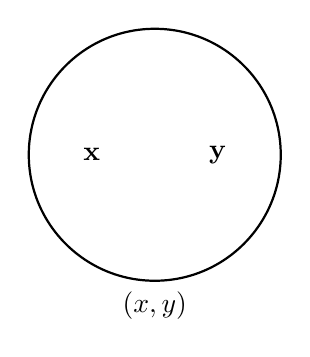
\begin{tikzpicture}[scale=0.8]
\draw[draw=black,thick](0,0)circle(2 and 2);
\draw(-1,0)node{\textbf{x}};
\draw(1,0)node{\textbf{y}};
\node[anchor=north] at (current bounding box.south) {$\partOf(x,y)$};
\end{tikzpicture}
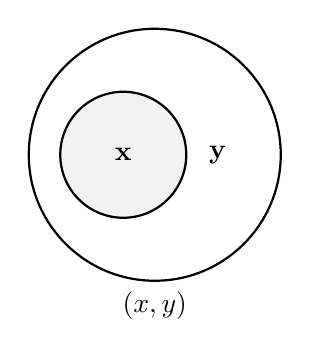
\begin{tikzpicture}[scale=0.8]
\draw[draw=black,thick](0,0)circle(2 and 2);
\draw[fill=gray!10,draw=black,thick](-0.5,0)circle(1 and 1);
\draw(-0.5,0)node{\textbf{x}};
\draw(1,0)node{\textbf{y}};
\node[anchor=north] at (current bounding box.south) {$\properPartOf(x,y)$};
\end{tikzpicture}
\end{center}
\caption{Simple vs. Proper Parthood}
\label{figure:SchematicProperPart}
\end{figure}
This Venn-style diagram depicts two scenarios:
\begin{description}
\item[\partOf(x,y)]
$x$ may be a part of $y$ or vice-versa;
$x$ and $y$ cannot be distinguished
\item[\properPartOf(x,y)] 
$x$ is certainly a part of $y$, however $y$ is not a part of $x$
\end{description} 
In general proper \gls{Parthood} is a asymmetric relationship:
\begin{align*}
&\properPartOf(x,y) 
\Rightarrow
\neg \properPartOf(y,x).
\qquad\text{\cite{DBLP:journals/dke/Varzi96} \cite{SEP:Mereology}}
&\text{Asymmetry}
\end{align*}

In this thesis and the remaining axioms, we tend towards the terminology used by \gls{Mereology} for \gls{Parthood} relations, which provides a clear tool-set for distinguishing part-whole relationships.
For instance, \gls{Mereology} also allows for the notion of atomicity, i.e. atomic parts which cannot be decomposed in further parts:
\begin{align*}
\atomicPart(x)
\Leftarrow
\not \exists p.\properPartOf(p,x).
\qquad\text{\cite{DBLP:journals/dke/Varzi96} \cite{SEP:Mereology}}
\end{align*}
Atomicity is later used to distinguish cases for \gls{Correspondence} and \gls{Conformance} (see §\ref{subsection:Correspondence} and §\ref{subsection:Conformance}).

\subsection{Fragments}
\label{subsection:Fragments}
\Glspl{Fragment} are a specialization of entities intended to capture the endogenous, mereological decomposition of artifacts \cite{DBLP:conf/modelsward/HeinzLV17}.
Axiom \ref{axiom:Fragment} defines  \glspl{Fragment} as artifacts, which are neither files nor folders, and are properly embedded in at least one other artifact.
For instance, consider the syntactical decomposition of \gls{Java} classes, i.e. the class \gls{Fragment} contains method and field \glspl{Fragment}.
\begin{axiom}[\Fragment]
\label{axiom:Fragment}
\begin{align*}
&\Fragment(f) 
\Rightarrow
\Artifact(a) \wedge \neg(\File(f) \vee \Folder(f)).\\
&\Fragment(f) 
\Rightarrow 
\exists a.\Artifact(a) \wedge \properPartOf(f,a).
\end{align*}
\end{axiom}
We emphasize the proper \gls{Parthood} here for reasons mentioned in §\ref{subsection:Parthood}.
If we were to use reflexive \gls{Parthood} for the definition of the \Fragment-predicate it would be a tautology:
\begin{align*}
&\Fragment(f) 
\Rightarrow 
\exists a.\Artifact(a) \wedge \partOf(f,a).
&\text{Tautology}
\end{align*}
Since $\Fragment(f)$ implies $\Artifact(f)$ and \partOf~ is reflexive, there exists always an artifact for a \gls{Fragment} the latter is a part of, which is the \gls{Fragment} itself.

From the specification of \glspl{Fragment} we can specialize the proper \gls{Parthood} predicate for \glspl{Fragment}:
\begin{align*}
&\fragmentOf(f,x) 
\Rightarrow
\Fragment(f) \wedge \Artifact(x).\\
&\fragmentOf(f,x) 
\Leftarrow
\Fragment(f) \wedge \Artifact(x) \wedge \properPartOf(f,x).
\end{align*}
This is just a restriction of domain and range facilitating a special semantic.
A \fragmentOf-relationship is not explicitly formalized in works on \glspl{LinguisticArchitecture}, i.e. \cite{DBLP:conf/sle/Lammel16} \cite{DBLP:conf/modelsward/HeinzLV17}.

We can also describe the process of fragmentation:
\begin{align*}
\partOf(p,w) \wedge \Fragment(w)
\Rightarrow
\Fragment(p).
\qquad
\text{\cite{DBLP:conf/modelsward/HeinzLV17}}
\end{align*}
The \gls{Fragment} nature propagates top-down alongside the order of \gls{Parthood}, i.e. if an entity is a \gls{Fragment} all parts are also \glspl{Fragment} \cite{DBLP:conf/modelsward/HeinzLV17}.

\subsection{Correspondence}
\label{subsection:Correspondence}
\Gls{Correspondence} is the relationship between to \glspl{Artifact} denoting both represent the same data in the sense that they are mereologically similar \cite{DBLP:conf/modelsward/HeinzLV17}.
It usually occurs as exogenous relationship, i.e. the involved \glspl{Artifact} do not belong to the same \gls{Language}, for instance \gls{XML} and \gls{JSON} may contain the same information.

In order to axiomatize \gls{Correspondence} properly we need to introduce two other relationships first, which are not explicitly defined in \cite{DBLP:conf/modelsward/HeinzLV17}:
\begin{description}[align=left]
\item[\represents]
The relationship denoting that an \gls{Artifact} is a \gls{Representation} or \gls{Manifestation} of an entity.
\begin{align*}
&\represents(a,e)
\Rightarrow
\Artifact(a) \wedge \Entity(e).\\
&\represents(a,e)
\Leftarrow
a \text{ is a representation of } e.
\end{align*}

\item[\sameAs]
The relationship denoting two artifacts represent the same entity.
\begin{align*}
&\sameAs(x,y)
\Rightarrow
\Artifact(x) \wedge \Artifact(y).\\
&\sameAs(x,y)
\Leftarrow
\exists e.\represents(x,e) \wedge \represents(y,e).
\end{align*}
\end{description}

The axiomatization of \gls{Correspondence} from \cite{DBLP:conf/modelsward/HeinzLV17} is slightly altered with emphasis of irreflexive proper \gls{Parthood}, see §\ref{subsection:Parthood}.
\begin{axiom}[\correspondsTo]
\label{axiom:CorrespondsTo}
~\newline
\resizebox{\linewidth}{!}{
\begin{minipage}{\linewidth}
\begin{align*}
\correspondsTo(x,y)
&\Rightarrow
\Artifact(x) \wedge \Artifact(y).\\
\correspondsTo(x,y)
&\Leftarrow
(\forall px.\properPartOf(px,x) \Rightarrow \exists py.\properPartOf(py,y) \wedge \correspondsTo(px,py))\\
&\wedge
(\forall py.\properPartOf(py,y) \Rightarrow \exists px.\properPartOf(px,x) \wedge \correspondsTo(py,px))\\
&\vee
(\not\exists p.\properPartOf(p,x) \vee \properPartOf(p,y)) \wedge \sameAs(x,y).
\end{align*}
\end{minipage}
}
\end{axiom}
Axiom \ref{axiom:CorrespondsTo} defines \gls{Correspondence} recursively:
\begin{enumerate}[align=left,label=\textbf{Case \Roman*},ref={\Roman*}]
\item
If both \glspl{Artifact} is atomic in the sense it cannot be decomposed in further parts, we check whether both artifacts represent the same data.

\item
Else, if at least one \gls{Artifact} is not atomic, then for each proper part of one \gls{Artifact} has to be a corresponding part in the other and vice versa.
\end{enumerate}
This axiomatization demands a strict one-to-one \gls{Correspondence} in its recursive clause which occurs in reflexive cases, i.e. $\correspondsTo(x,x)$.
A strict one-to-one \gls{Correspondence} may be to strict for real-world applications \cite{DBLP:conf/sle/Lammel16}.
\Gls{Correspondence} inherits transitivity from \represents~ and \properPartOf.

\subsection{Conformance}
\label{subsection:Conformance}
\Gls{Conformance} is the relationship between two \glspl{Artifact} denoting one satisfies the specification given by the other \cite{DBLP:conf/modelsward/HeinzLV17}.
This satisfaction is also meant to be mereologically decomposable, i.e. there are parts of one \gls{Artifact} specified by a part of the other.


In order to axiomatize \gls{Conformance} properly we need to introduce two other relationships first.
Both relations are not formalized in \cite{DBLP:conf/modelsward/HeinzLV17} as they are here:
\begin{description}[align=left]
\item[\defines]
The relationship simply denoting an \gls{Artifact} contains the definition of an entity.
\begin{align*}
\defines(a,e)
&\Rightarrow
\Artifact(a) \wedge \Entity(e).\\
\defines(a,e)
&\Leftarrow
a \text{ is a definition for } e.
\end{align*}

\item[\elementOf]
The relationship denoting set-theoretic membership.\footnote{We do not use the \elementOf~ axiom for \glspl{Artifact} and \glspl{Language} from \cite{DBLP:conf/modelsward/HeinzLV17}, because it introduces the possibility for infinite mutual recursion:
\begin{align*}
\elementOf(a,l)
&\Rightarrow
\Artifact(a) \wedge \Language(l).\\
\elementOf(a,l)
&\Leftarrow
\exists s.\defines(s,l) \wedge \conformsTo(a,s)
\end{align*}}
\begin{align*}
\elementOf(e,s)
&\Rightarrow
\Entity(e) \wedge \Set(s).\\
\elementOf(e,s)
&\Leftarrow
e \in s.
\end{align*}


\end{description}


The axiomatization of \gls{Conformance} from \cite{DBLP:conf/modelsward/HeinzLV17} is also slightly altered with emphasis of irreflexive proper \gls{Parthood}; reasons for this are mentioned in §\ref{subsection:Parthood}.
\begin{axiom}[\conformsTo]
\label{axiom:ConformsTo}
~\newline
\resizebox{\linewidth}{!}{
\begin{minipage}{\linewidth}
\begin{align*}
\conformsTo(a,d)
&\Rightarrow
\Artifact(a) \wedge \Artifact(d).\\
\conformsTo(a,d)
&\Leftarrow
(\forall pa.\properPartOf(pa,a) \wedge \exists pd.\properPartOf(pd,d) \wedge \conformsTo(pa,pd))\\
&\vee \exists l.\defines(d,l) \wedge \elementOf(a,l).
\end{align*}
\end{minipage}
}
\end{axiom}
Axiom \ref{axiom:ConformsTo} defines \gls{Conformance} recursively:
\begin{enumerate}[align=left,label=\textbf{Case \Roman*},ref={\Roman*}]
\item
If both \glspl{Artifact} is atomic in the sense it cannot be decomposed in further parts, we check whether one \gls{Artifact} defines a language the other \gls{Artifact} is an element of.

\item
Else, if at least one \gls{Artifact} is not atomic, then for each proper part of one \gls{Artifact} has to be a proper part in the other \gls{Artifact} it conforms to.
\end{enumerate}


\section{Traceability}
\label{section:Traceability}
This section provides brief background on the topic of \gls{Traceability}, i.e. its objectives and terminology (see §\ref{subsection:TraceabilityObjectives} and §\ref{subsection:TraceabilityTerminology} respectively).

\subsection{Traceability Objectives}
\label{subsection:TraceabilityObjectives}
\Gls{Traceability}, as a desired property of software systems and their development processes, originates from requirement engineering, i.e.
how do we validate or verify that all requirements are met;
or more precisely: on what data can we base such validation or verification?
\cite{DBLP:journals/sosym/WinklerP10}

An answer to these questions is motivated by observations on development processes of software systems.
Because such a process usually has an iterative and incremental nature, we can reasonably assume engineering activities to leave \glspl{Trace} which reflect the performed action.

Modern day \gls{Traceability} objectives are not limited to validation of requirement compliance.
It is also regarded as a desirable property for supporting engineering activities, e.g. change impact analysis or dependency analysis \cite{DBLP:books/daglib/p/GotelCHZEGDAMM12} \cite{DBLP:conf/re/GotelF94}.
This feeds to the overall topic of program comprehension.
We can informally define \gls{Traceability} as \textit{"[...] the ability to [...] interrelate uniquely identifiable
entities in a way that matters."} \cite{PaigeOKZPC2010} \cite{DBLP:journals/sosym/WinklerP10}.


\subsection{Traceability Terminology}
\label{subsection:TraceabilityTerminology}
This section recapitulates the necessary excerpt of definitions on \gls{Traceability} terms given by \cite{DBLP:books/daglib/p/GotelCHZEGDAMM12}.
An excessive glossary of \gls{Traceability} terminology can be found in \cite{TraceabilityGlossary}.

\begin{definition}[Trace]
~
\begin{itemize}
\item
\textbf{(Noun)}
A specified triplet of elements comprising: a source artifact, a target artifact and a trace link associating the two artifacts.
\cite{DBLP:books/daglib/p/GotelCHZEGDAMM12}

\item
\textbf{(Verb)}
The act of following a trace link from a source artifact to a target artifact or vice-versa.
\cite{DBLP:books/daglib/p/GotelCHZEGDAMM12}
\end{itemize}
\end{definition}

\begin{definition}[Trace Artifact, Source Artifact, Target Artifact]
A traceable unit of da\-ta (e.g., a single requirement, a cluster of requirements, a UML class, a UML class operation, a Java class or even a person).
A trace artifact is one of the trace elements and is qualified as either a source artifact or as a target artifact when it participates in a trace:
\begin{itemize}
\item
\textbf{Source Artifact}
The artifact from which a trace originates.
\item
\textbf{Target Artifact}
The artifact at the destination of a trace.
\end{itemize}
\cite{DBLP:books/daglib/p/GotelCHZEGDAMM12}
\end{definition}

\begin{definition}[Trace Artifact Type]
A label that characterizes those trace artifacts that have the same or a similar structure (syntax) and/or purpose (semantics).
For example, requirements, design and test cases may be distinct artifact types.
\cite{DBLP:books/daglib/p/GotelCHZEGDAMM12}
\end{definition}

\begin{definition}[Trace Link]
A specified association between a pair of artifacts, one comprising the source artifact and one comprising the target artifact. 
Trace links are effectively bidirectional. 
\cite{DBLP:books/daglib/p/GotelCHZEGDAMM12} 
\end{definition}

\begin{definition}[Trace Link Type]
A label that characterizes those trace links that have the
same or similar structure (syntax) and/or purpose (semantics). 
For example, “implements”, “tests”, “refines” and “replaces” may be distinct trace link types. 
\cite{DBLP:books/daglib/p/GotelCHZEGDAMM12} 
\end{definition}

\begin{definition}[Traceability]
The potential for traces to be established and used.
Traceability (i.e., trace “ability”) is thereby an attribute of an artifact or of a collection of artifacts.
\cite{DBLP:books/daglib/p/GotelCHZEGDAMM12} 
\end{definition}

\begin{definition}[Traceability Creation]
The general activity of associating two (or more) artifacts, by providing trace links between them. 
This can be done manually, automatically or semi-automatically, and additional annotations can be provided as desired to characterize attributes of the traces.
\cite{DBLP:books/daglib/p/GotelCHZEGDAMM12}
\end{definition}

\begin{definition}[Trace Recovery]
A particular approach to trace creation that implies the creation of trace links after\footnote{The opposite to trace recovery is \textbf{Trace Capture}: \textit{"A particular approach to trace creation that implies the creation of trace links concurrently with the creation of the artifacts that they associate. These trace links may be created automatically or semi-automatically using tools."}\cite{DBLP:books/daglib/p/GotelCHZEGDAMM12}. This is similar to the distinction between \gls{StaticProgramAnalysis} and dynamic program analysis, thus leaving the scope of this thesis.} the artifacts that they associate have been generated and manipulated.
These trace links may be created automatically or semi-automatically using tools. 
\cite{DBLP:books/daglib/p/GotelCHZEGDAMM12}
\end{definition}


\section{Technological Background}
This section provides background on key \glspl{Technology} used by this thesis.
§\ref{subsection:MegaLXText} introduces the \gls{MegaL} modeling language and \gls{MegaL/Xtext} as corresponding technology.
§\ref{subsection:JAXB} and §\ref{subsection:Hibernate} provides an introduction to \gls{JAXB} and \gls{Hibernate} respectively.
§\ref{subsection:ANTLR} summarizes the relevant aspects of \gls{ANTLR}.

\subsection{MagaL \& MegaL/Xtext}
\label{subsection:MegaLXText}
\gls{MegaL} \cite{DBLP:conf/ecmdafa/LammelV14} \cite{DBLP:conf/models/FavreLV12} is a modeling language for \glspl{LinguisticArchitecture} developed by Software Languages Team\footnote{\url{http://www.softlang.org/}(Retrieved \formatdate{12}{12}{2017})} at the University of Koblenz-Landau.
\gls{MegaL/Xtext} \cite{LukasHaertelBScThesis} \cite{HaertelHHLV17} is the integration of \gls{MegaL} into the eclipse \gls{IDE} based on Xtext\footnote{\url{http://www.eclipse.org/Xtext/}(Retrieved \formatdate{12}{12}{2017})} developed by the same team.

\Gls{MegaL} provides a textual notation for typed \glspl{ERModel}, i.e. each entity and each relation is strictly typed.
This is exemplified by listing \ref{listing:AMegamodelForCitation} showing a simple \gls{Megamodel} for citation of scientific papers.
\begin{lstlisting}[caption={A Megamodel for Citation},label={listing:AMegamodelForCitation}]
Artifact < Entity
File < Artifact
Paper < File

cites < Paper * Paper

paper1 : Paper
paper2 : Paper
paper1 cites paper2
\end{lstlisting}
The types, starting with upper-case letters, state that there are files, which are papers.
There is a relation \texttt{cites}, denoted with a type signature, stating one paper may cite the other.
Eventually, there are two concrete paper entity instances \texttt{paper1} and \texttt{paper2}, where the former cites the latter instance.

\Gls{MegaL/Xtext} provides means for applying additional functionality or semantics to \glspl{Megamodel}, e.g. for reasoning or validation on the induced entity graph.
For this, \gls{MegaL/Xtext} implements a plug-in system, which is exemplified with the following listings \ref{listing:MegalXtextPluginIntegration}, \ref{listing:MegaLXtextGuidedReasonerPluginBaseClass} and \ref{listing:MegaLXtextGuidedReasonerPluginDerivedClass}.
\begin{lstlisting}[caption={MegaL/Xtext Plugin Integration},label={listing:MegalXtextPluginIntegration}]
MyType < Entity

@Plugin 'MyRelationPlugin'
myRelation < MyType * MyType

MyRelationPlugin : Plugin
MyRelationPlugin = 'classpath:org.softlang.megal.MyRelationPlugin'
\end{lstlisting}
\begin{lstlisting}[language=Java,caption={MegaL/Xtext GuidedReasonerPlugin base class},label={listing:MegaLXtextGuidedReasonerPluginBaseClass}]
public abstract class GuidedReasonerPlugin extends InjectedReasonerPlugin {
	...
	protected void guidedDerive(EntityType entityType) throws Throwable {}
	protected void guidedDerive(RelationshipType relationshipType) throws Throwable {}
	protected void guidedDerive(Entity entity) throws Throwable {}
	protected void guidedDerive(Relationship relationship) throws Throwable {}
}
\end{lstlisting}
\begin{lstlisting}[language=Java,caption={MegaL/Xtext GuidedReasonerPlugin derived class},label={listing:MegaLXtextGuidedReasonerPluginDerivedClass}]
public class MyRelationPlugin extends GuidedReasonerPlugin {
	protected void guidedDerive(Relationship relationship) throws Throwable {
		...
	}
}
\end{lstlisting}
Given a \gls{Java} class \gls{Artifact} \texttt{MyRelationPlugin.java} implementing special features provided by the \gls{MegaL/Xtext} \gls{API}, e.g. the \texttt{GuidedReasonerPlugin} class, it can be bound to an entity instance by using its classpath.
This plug-in entity can then be used with the \texttt{@Plugin} annotation and applied to \gls{MegaL} elements, i.e. entity types, relationship types, entity instances and relationship instances.
\texttt{MyRelationPlugin} will be executed during evaluation of the \gls{Megamodel}.


\subsection{JAXB (Java Architecture for XML Binding)}
\label{subsection:JAXB}
\Gls{JAXB} \cite{JAXB} \cite{JAXBTutorial}
is a \gls{Java} technology developed by the Oracle Corporation for \gls{XML} serialization and de-serialization of classes and instances.
It implements \gls{O/X-Mapping}, i.e. \gls{Java} classes can be transformed to \gls{XML} schema files (\gls{XSD} files) and instances of classes can be transformed to \gls{XML} documents.
Transformations can also be applied vice-versa.
Figure \ref{figure:JAXBDataBindingProcess} shows the \gls{O/X-Mapping} facilitated by \gls{JAXB}.
\begin{figure}[h!]
\begin{center}
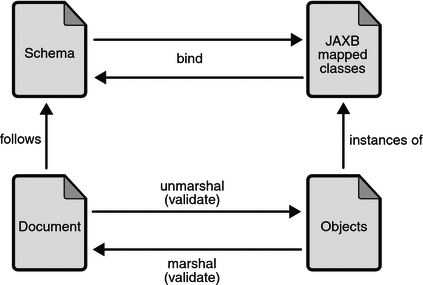
\includegraphics[width=\textwidth]{images/jaxb-dataBindingProcess_gray.png}
\end{center}
{
\scriptsize
\begin{center}
This image is taken from \cite{jaxbDataBindingProcess}:\\
\url{https://docs.oracle.com/javase/tutorial/figures/jaxb/jaxb-dataBindingProcess.gif}\\
(retrieved \formatdate{11}{12}{2017})
\end{center}
}
\caption{Steps in the JAXB Binding Process}
\label{figure:JAXBDataBindingProcess}
\end{figure}
The mapping of classes to schemas is called \textit{binding}, whereas the mapping of instances to documents is called \textit{marshaling} or \textit{unmarshaling} respectively.

Binding and marshaling is defined through \gls{Java} annotations.
For instance, class and field declarations can be annotated to specify marshaling into specific syntactic \gls{XML} elements, i.e. element tags or attributes.
This is exemplified by listing \ref{listing:AJAXBAnnotatedClass}:
\begin{lstlisting}[language=Java,caption={A JAXB annotated class},label={listing:AJAXBAnnotatedClass}]
@XmlRootElement(name="employee")
@XmlAccessorType(XmlAccessType.FIELD)
public class Employee {
	@XmlAttribute private int id;
	...
}
\end{lstlisting}
Annotations can define binding in more detail than shown above, e.g. it is possible to explicitly provide names and types of \gls{XML} elements.
Marshaling itself is triggered using reflection and the \texttt{JAXBContext} class:
\begin{lstlisting}[language=Java,caption={JAXB marshaling in Java},label={listing:JAXBMarshalingInJava}]
JAXBContext context = JAXBContext.newInstance(Employee.class);
context.createMarshaller().marshal(jaxbElement, writer);
\end{lstlisting}
More excessive examples and tutorials on \gls{JAXB} can be found in \cite{JAXB} and in \cite{JAXBTutorial}.

\subsection{Hibernate}
\label{subsection:Hibernate}
\gls{Hibernate} \cite{HibernateORM} is a \gls{Java} technology developed by Red Hat Inc. facilitating \gls{O/R-Mapping}.
Using \gls{Hibernate}, one can define mappings from \gls{Java} classes and their instances to tables of relational databases and their rows, and vice versa.
This allows the underlying framework to generate \gls{SQL} code for communicating with a relational database system in order to provide means for CRUD operations.

Mappings can be defined using \gls{JPA} annotations or, traditionally, using \gls{XML} files, i.e. for each \gls{Java} class file \texttt{MyEntity.java} representing a data entity exists a mapping file \texttt{MyEntity.hbm.xml} describing the relational mapping.
This is exemplified by the following two listings \ref{listing:ExcerptOfTheEmployeeJavaClass} and \ref{listing:ExcerptOfTheEmployeeHibernateMappingFile}:
\begin{lstlisting}[language=Java,caption={Excerpt of the Employee Java class},label={listing:ExcerptOfTheEmployeeJavaClass}]
public class Employee {
	private int id;
	...
}
\end{lstlisting}
\begin{lstlisting}[language=Xml,caption={Excerpt of the Employee Hibernate mapping file},label={listing:ExcerptOfTheEmployeeHibernateMappingFile}]
<class name="Employee" table="EMPLOYEES">
	<id name="id" column="EMPLOYEE_ID">
	    ...
	</id>
    ...	
</class>
\end{lstlisting}
Here, the \texttt{Employee} class is mapped to the \texttt{EMPLOYEE} table its \texttt{id} field is mapped to the \texttt{EMPLOYEE\_ID} column as primary key for the table. More excessive examples and tutorials on \gls{Hibernate} can be found in \cite{HibernateORM}.


\subsection{ANTLR (Another Tool For Language Recognition)}
\label{subsection:ANTLR}
\Gls{ANTLR} \cite{Parr:2013:DAR:2501720} is a technology providing means for processing structured text using parsing.
It is available for \gls{Java}, C\#, JavaScript, Python and many other platforms \cite{antlr.org}, i.e. \Gls{ANTLR} can generate $LL(*)$ parsers for context-free languages in the target platform's language.
Parsers are generated from an EBNF-like grammar notation, e.g. the following "hello"-grammar in listing \ref{listing:TheHelloANTLRGrammar} taken from \cite{ANTLRv4GettingStarted}:
\begin{lstlisting}[caption={The Hello ANTLR grammar},label={listing:TheHelloANTLRGrammar}]
grammar Hello;
hello  : 'hello' ID ;     // match keyword hello followed by an identifier
ID : [a-z]+ ;             // match lower-case identifiers
WS : [ \t\r\n]+ -> skip ; // skip spaces, tabs, newlines
\end{lstlisting}

\Gls{ANTLR} also provides means for integrating generated parsers into one's pro\-ject, i.e. means for working with/traversing created \glspl{ParseTree}.
Tree traversal in order to transform \glspl{ParseTree} to \glspl{AST} can be either done traditionally using the \gls{VisitorPattern} or using the combination of \gls{ANTLR} \gls{ParseTree} walkers and walker listeners, a variation of the \gls{ObserverPattern}.

Listener interfaces are generated during parser generation.
All listeners implement the \texttt{ParseTreeListener} interface provided by the \gls{ANTLR} runtime.
The interface is shown in \ref{listing:TheANTLRParseTreeListenerInterface}.
\begin{lstlisting}[language=Java,caption={The ANTLR ParseTreeListener interface},label={listing:TheANTLRParseTreeListenerInterface}]
public interface ParseTreeListener {
	void visitTerminal(TerminalNode node);
	void visitErrorNode(ErrorNode node);
	void enterEveryRule(ParserRuleContext ctx);
	void exitEveryRule(ParserRuleContext ctx);
}
\end{lstlisting}
Listing \ref{listing:AnExtensionOftheANTLRParseTreeListenerInterface} shows the generated listener interface for the grammar above.
\begin{lstlisting}[language=Java,caption={An extension of the ANTLR ParseTreeListener interface},label={listing:AnExtensionOftheANTLRParseTreeListenerInterface}]
public interface HelloListener extends ParseTreeListener {
    void enterHello(HelloContext ctx);
    void exitHello(HelloContext ctx);
}
\end{lstlisting}
While traversing a \gls{ParseTree}, listeners are notified upon entering or exiting tree nodes, called "context" by \gls{ANTLR}.
Traversal is triggered using \texttt{Parse\-Tree\-Walker} instances, which implement \gls{DFS}.
Usage of \texttt{Parse\-Tree\-Walker} is exemplified in listing \ref{listing:ApplicationOfTheANTLRParseTreeWalker}.
\begin{lstlisting}[language=Java,caption={Application of the ANTLR ParseTreeWalker},label={listing:ApplicationOfTheANTLRParseTreeWalker}]
...
HelloListener helloListener = ...
ParseTreeWalker parseTreeWalker = new ParseTreeWalker();
parseTreeWalker.walk(helloListener, parseTree);
...
\end{lstlisting}

An excessive introduction to \gls{ANTLR} can be found in \cite{Parr:2013:DAR:2501720}, a simple tutorial can be found in \cite{ANTLRv4GettingStarted}.